%%%%%%%%%%%%%%%%%%%%%%%%%%
%                        %
% Luther Michaels        % 
% ECE 351-52             %
% Lab 9                  %
% November 4, 2021       %
% Fast Fourier Transform %
%             Lab Report %
%                        %
%%%%%%%%%%%%%%%%%%%%%%%%%%

%%%%%%%%%%%%%%%%%%%%%%%%%%%%%%%%%%%%%%%%%%%
%%% DOCUMENT PREAMBLE %%%
\documentclass[12pt]{report}
\usepackage[english]{babel}
\usepackage{url}
\usepackage[utf8x]{inputenc}
\usepackage{amsmath}
\usepackage{graphicx}
\graphicspath{{images/}}
\usepackage{parskip}
\usepackage{fancyhdr}
\usepackage{vmargin}
\usepackage{listings}
\usepackage{hyperref}
\usepackage{xcolor}

\definecolor{codegreen}{rgb}{0,0.6,0}
\definecolor{codegray}{rgb}{0.5,0.5,0.5}
\definecolor{codeblue}{rgb}{0,0,0.95}
\definecolor{backcolour}{rgb}{0.95,0.95,0.92}

\lstdefinestyle{mystyle}{
	backgroundcolor=\color{backcolour},   
	commentstyle=\color{codegreen},
	keywordstyle=\color{codeblue},
	numberstyle=\tiny\color{codegray},
	stringstyle=\color{codegreen},
	basicstyle=\ttfamily\footnotesize,
	breakatwhitespace=false,         
	breaklines=true,                 
	captionpos=b,                    
	keepspaces=true,                 
	numbers=left,                    
	numbersep=5pt,                  
	showspaces=false,                
	showstringspaces=false,
	showtabs=false,                  
	tabsize=2
}

\lstset{style=mystyle}

\setmarginsrb{3 cm}{2.5 cm}{3 cm}{2.5 cm}{1 cm}{1.5 cm}{1 cm}{1.5 cm}

\title{9}	% Title						
\author{Luther Michaels}	% Author		
\date{November 4, 2021}   % Date

\makeatletter
\let\thetitle\@title
\let\theauthor\@author
\let\thedate\@date
\makeatother

\pagestyle{fancy}
\fancyhf{}
\rhead{\theauthor}
\lhead{\thetitle}
\cfoot{\thepage}
%%%%%%%%%%%%%%%%%%%%%%%%%%%%%%%%%%%%%%%%%%%%

\begin{document}
	
%%%%%%%%%%%%%%%%%%%%%%%%%%%%%%%%%%%%%%%%%%%%%%%%%%%%%%%%%%%%%%%%%%%%%%%%%%%%%%%%%%
%%% TITLE PAGE %%%
\begin{titlepage}
	\centering
	\vspace*{0.5 cm}
		
	\begin{center}    
		\textsc{\Large   ECE 351 - Section \#52}\\[2.0 cm]	
	\end{center}  
	\textsc{\Large Fast Fourier Transform  }\\[0.5 cm]
	\rule{\linewidth}{0.2 mm} \\[0.4 cm]
	{ \huge \bfseries \thetitle}\\
	\rule{\linewidth}{0.2 mm} \\[1.5 cm]
	\begin{minipage}{0.4\textwidth}
		\begin{flushleft} \large
		\end{flushleft}
	\end{minipage}~
	\begin{minipage}{0.4\textwidth}
		\begin{flushright} \large
			\emph{Submitted By:} \\
			Luther Michaels \break
			
			\emph{Submission Date:} \\
			November 4, 2021
		\end{flushright}
	\end{minipage}\\[2 cm]
\end{titlepage}
	
%%%%%%%%%%%%%%%%%%%%%%%%%%%%%%%%%%%%%%%%%%%%%%%%%%%%%%%%%%%%%%%%%%%%%%%%%%%%%%%%%%
%%% TABLE OF CONTENTS %%%

\tableofcontents
\pagebreak

%%%%%%%%%%%%%%%%%%%%%%%%%%%%%%%%%%%%%%%%%%%%%%%%%%%%%%%%%%%%%%%%%%%%%%%%%%%%%%%%%%
%%% LAB REPORT %%%
\renewcommand{\thesection}{\arabic{section}}
\section{Introduction}
		  
The main concept explored in this lab is the process of taking fast Fourier transforms with Python. The goal is to create a user-defined function that implements a fast Fourier transform routine in order to obtain the frequency domain components of its input. The resultant magnitude and phase over the frequency range can then be plotted for an input function. \\

The fast Fourier transform is an established method of computing the Fourier transform of an input and can be utilized via Python packages. The function scipy.fftpack.fft() returns the Fourier transform and scipy.fftpack.fftshift() shifts the zero frequencies and corresponding points to its center. In order to plot the frequency domain magnitudes and phases found with this system, the function matplotlib.pyplot.stem() is needed. A specified range may be viewed by limiting the x-axis of a plot with matplotlib.pyplot.xlim(). This procedure will require the use of the series derived and defined in Lab 8. All output and plots can be produced through Python implementation written within the Spyder software. \\

\section{Equations}

\begin{equation}
	x_1(t) = cos(2\pi t)
\end{equation}
\begin{equation}
	x_2(t) = 5sin(2\pi t)
\end{equation}
\begin{equation}
	x_3(t) = 2cos((2\pi \cdot 2t) - 2) + sin^2((2\pi \cdot 6t) + 3)
\end{equation}
\begin{equation}
	x_4(t) = \sum_{k=1}^{N}\frac{2}{k\pi}[1 - cos(k\pi)]sin(\frac{2\pi kt}{T})
\end{equation}
\begin{equation*}
	\mathcal{F}\{cos(2\pi f_0t)\} = \frac{1}{2}[\delta(f - f_0) + \delta(f + f_0)]
\end{equation*}
\begin{equation}
	\mathcal{F}\{cos(2\pi t)\} = \frac{1}{2}[\delta(f - 1) + \delta(f + 1)]
\end{equation}
\begin{equation*}
	\mathcal{F}\{sin(2\pi f_0t)\} = \frac{1}{j2}[\delta(f - f_0) - \delta(f + f_0)]
\end{equation*}
\begin{equation}
	\mathcal{F}\{5sin(2\pi t)\} = \frac{5}{j2}[\delta(f - 1) - \delta(f + 1)]
\end{equation}

\section{Methodology}

Prior to the first task, the lab procedure requested that a fast Fourier transform function be defined utilizing the provided code in the lab manual. This was accomplished by creating a function in Python and copying the code into the body. The input arguments were given as the function $ x(t) $ and the sampling frequency. A clean flag was also added to facilitate later functionality. The function would then return the frequency that had been arranged in addition to the obtained magnitude and phase values of the input $ x(t) $. \\ 

Task 1 required that this user-defined fast Fourier transform function be utilized to produce a plot combining five subplots for Equation 1. These plots would include: the original function, the magnitude, the phase, the magnitude focused only on relevant points, and the phase focused on relevant points. The step size was initialized to $ 1\times 10^{-2} $ for proper resolution, and the initial time domain interval defined from 0 to 2 seconds using numpy.arange(). This time interval was defined without the addition of the step variable to the upper limit. As this combination plot would be repeated in later tasks, a function was created for the sequence of commands needed to produce the individual subplots. \\

This plot function would accept seven arguments: the input function x(t), the setting of the clean condition, the x and y dimensions of the overall plot, the plot title, the x-axis limiting values, and the time interval. The frequency, magnitude, and phase would be obtained by calling the fast Fourier transform function on x(t) with a constant sampling frequency of $ 100 $ and clean flag within the plot function. The sequence would then proceed as in prior labs by declaring the plot size at the outset, arranging the subplot, plotting the relevant variables, and providing a title and axis labels as necessary. The matplotlib.pyplot.stem() function was utilized to plot all frequency domain subplots. The two focused subplots attained restricted x-axes by passing the x limit value to the matplotlib.pyplot.xlim() function. \\

Tasks 2 and 3 asked that Equations 2 and 3 be plotted in like manner to that of Equation 1. This was done by assigning each function and plot title to individual variables. These variables were then passed as arguments to the plot function detailed above, alongside the specific values needed for the other parameters. The overall plot size was chosen to prevent any labels from overlapping. The x-axis limits were determined by first plotting the function and identifying points of interest. In both tasks, the clean flag was set to zero. \\

Task 4 requested that the three plots in Tasks 1-3 be reproduced and modified slightly, changing the phase plots to be more visually clean. This was accomplished by modifying the original fast Fourier transform function to respond to a clean flag. If the clean flag was set, the function would iterate for all values of the phase, checking if the magnitude was below $ 1\times 10^{-10} $. Any time this condition was met, the phase would be zeroed out for the corresponding index of the frequency. With this addition, the plots were created using the same commands as in Tasks 1-3, but having set the clean flag in each plot function call. \\

The fifth task required that the series derived in Lab 8 and shown in Equation 4 be given as the input to the user-defined fast Fourier function with $ N = 15 $. The time interval was set between 0 and 16 seconds using numpy.arange(). The functions defined by Equation 4 from Lab 8 were then copied into the code with the only alteration being the inclusion of the T variable as a parameter to the series function. The series in Equation 4 was then assigned to a variable by calling this function for $ T = 8 $. This variable and the plot title were passed to the plot function along with the other conditions and a set clean flag. \\

Github Link: \url{https://github.com/Luther-Michaels} \\

\section{Results}

After creating a working fast Fourier transform function and a routine to create the five-subplot graph, the combined plot for Equation 1 was obtained as shown below. The five subplots are arranged in the order and placement requested with a title and appropriate labels. The step size has obtained good resolution and is not so small that the plots are visually indistinguishable. The time interval shown in the first subplot is properly set from $ 0 $ to $ 2s $. The time domain plot of the function clearly represents a cosine function with a period of $ 1 $ as indicated by Equation 1. The focused subplots on the lower right-hand side show that the x-axis has been limited as requested to display the relevant points from the corresponding plots on the left-hand side. The frequency domain magnitude is represented by two shifted delta functions of magnitude $ 0.5 $, as Equation 5 would suggest. The unclean plot of the phase is cluttered as to be expected. The result from this first task is supported by the fact that it matches the example shown in the lab manual for the same function. \\

\begin{center}
	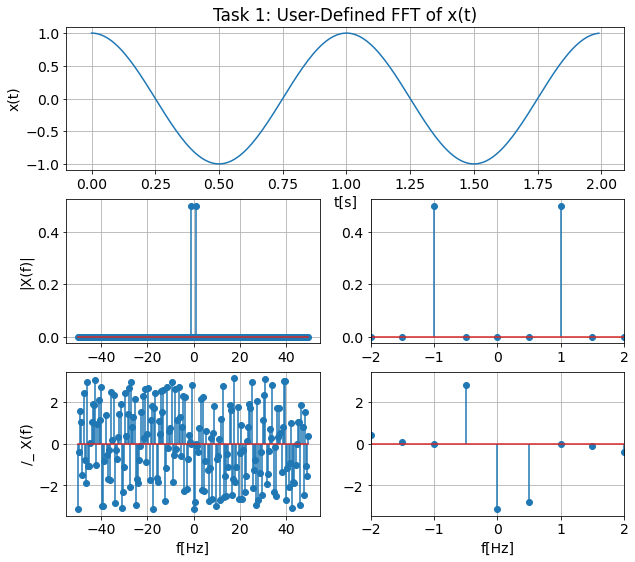
\includegraphics[scale = 0.38]{Lab 9 - Plots/Task1.png}\\[1.0 cm]
\end{center}

The combined plot of Equation 2 is shown next. The first subplot shows that the proper time interval has been retained, displaying a sine function with an amplitude of $ 5 $ and a period of $ 1 $ as is expected from the input function. The magnitude is given as two shifted positive delta functions of amplitude $ 2.5 $. This matches expectations given Equation 6, as the magnitude would take the absolute value to eliminate the negative sign. The x-axis limitations once again capture the relevant information shown in their counterparts, and the phase has not been cleaned. \\

\begin{center}
	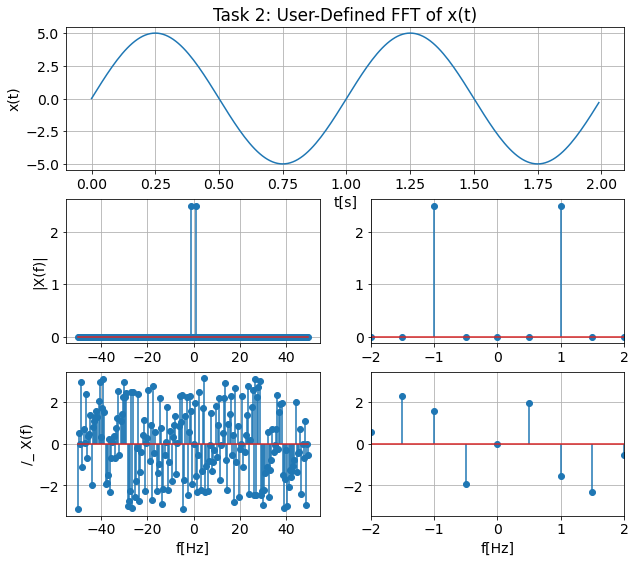
\includegraphics[scale = 0.38]{Lab 9 - Plots/Task2.png}\\[1.0 cm]
\end{center}

The five subplots for Equation 3 are gathered together in the following graph. The overall plot dimensions have been increased to display the y-axis labels with no overlap. While less intuitive than the prior functions, the plot of the input function in the time domain shows an addition of shifted cosine and sine terms to produce the sinusoidal signal we expect. In order to contain all the relevant points, the x-axis limits were properly set between $ -15 $ and $ 15 $ as shown. Both the original and the focused phase plots reveal the need to eliminate extraneous values for a more clean output.

\begin{center}
	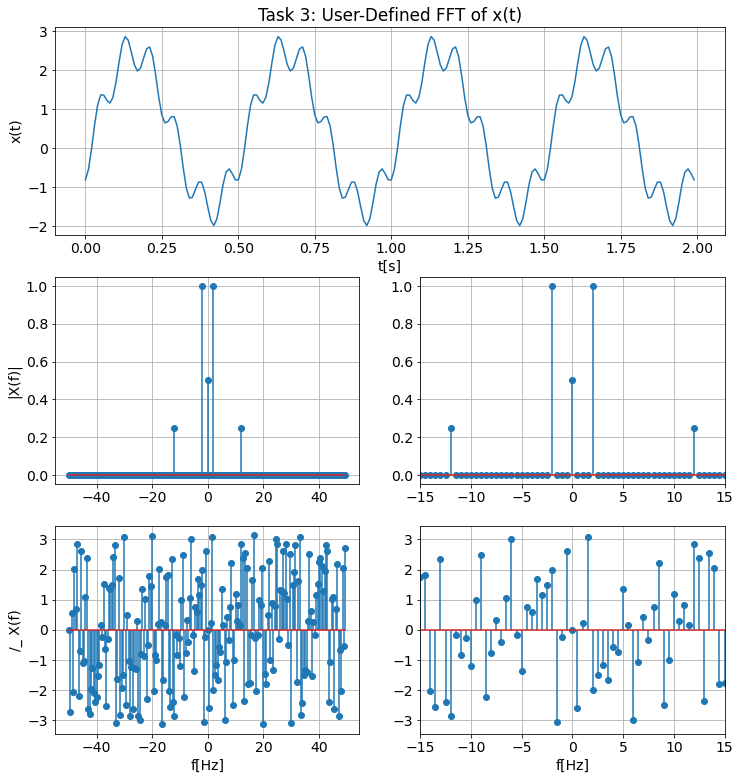
\includegraphics[scale = 0.4]{Lab 9 - Plots/Task3.png}\\[1.0 cm]
\end{center}

The cleaned up phase subplots for Equation 1 are shown below. As we should expect, all subplots but the two relating to the phase are identical to those produced in Task 1. The phase plots indicate that only two of the original lines resulted from points with magnitudes greater than $ 1\times 10^{-10} $. The x-axis limits are sufficient to capture these two relevant shapes. The other points in the original focused plot have been zeroed out. \\

\begin{center}
	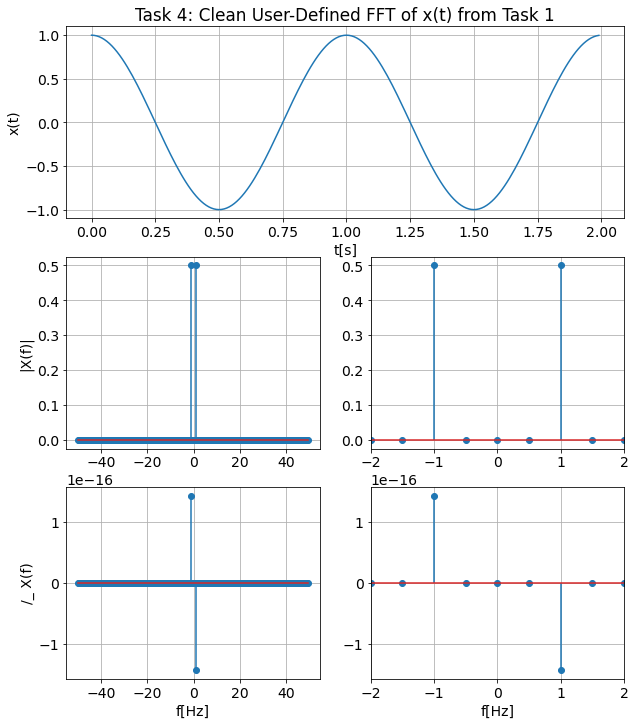
\includegraphics[scale = 0.35]{Lab 9 - Plots/Task4-1.png}\\[1.0 cm]
\end{center}

The plot of Equation 2 is shown next with the cleaned phase subplots. While the other subplots remain unchanged, the phase now displays only two lines as in the prior plot. As a result, both the phases are now shown identically to those for Equation 1. The two lines are properly displayed in the focused view, with zeros replacing all other original points. \\

\begin{center}
	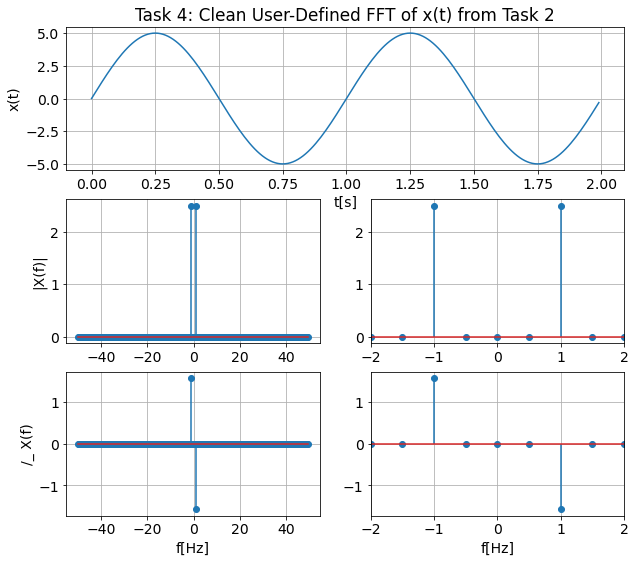
\includegraphics[scale = 0.37]{Lab 9 - Plots/Task4-2.png}\\[1.0 cm]
\end{center}

The phase plots that were cleaned for Equation 3 are shown in the following combined graph. As in both prior plots, all subplots have remained unchanged from the original appearance save the two involving the phase. Reviewing the unclean subplots, the results of the cleaning appear to closely correspond to the general trend of the many points displayed. This was also the case in the prior plots, though less pronounced. The four remaining lines have been captured within the focused bounds, with many of the original points visibly reduced to zero. All three of these cleaned plots have revealed the immense visual affect of points with magnitudes less than $ 1\times 10^{-10} $, while those points have little actual affect on the accuracy. \\

\begin{center}
	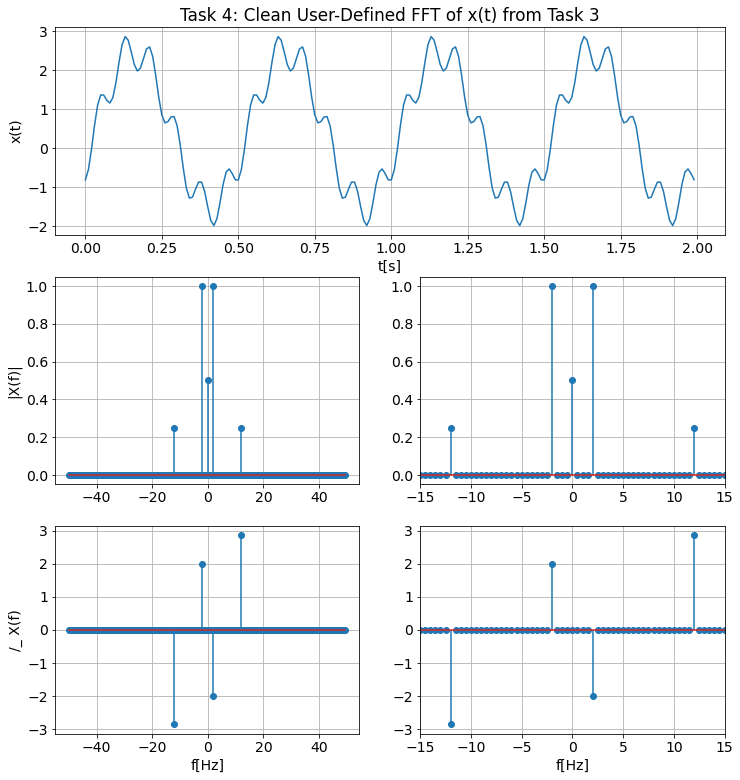
\includegraphics[scale = 0.4]{Lab 9 - Plots/Task4-3.png}\\[1.0 cm]
\end{center}

The combined plot of the series from Lab 8 given by Equation 4 is shown below with the cleaned phase subplots. As $ N = 15 $, the approximation of the square wave shown in the first time domain subplot is as accurate a representation as we would expect. The magnitude is presented as a series of shifted delta pairs that diminish outward. This makes sense given that both cosine and sine inputs were represented by two shifted delta functions and the summation would produce additional pairs of lesser magnitudes. The phase likewise matches our expectations given the plots from Equations 1 and 2. Those phase subplots showed a positive delta shifted left and a negative delta shifted right. The subplots for this series show a summation presented by multiple iterations of this sequence. The x-axis limits have been set to sufficiently display all relevant points in the focused subplots. \\

\begin{center}
	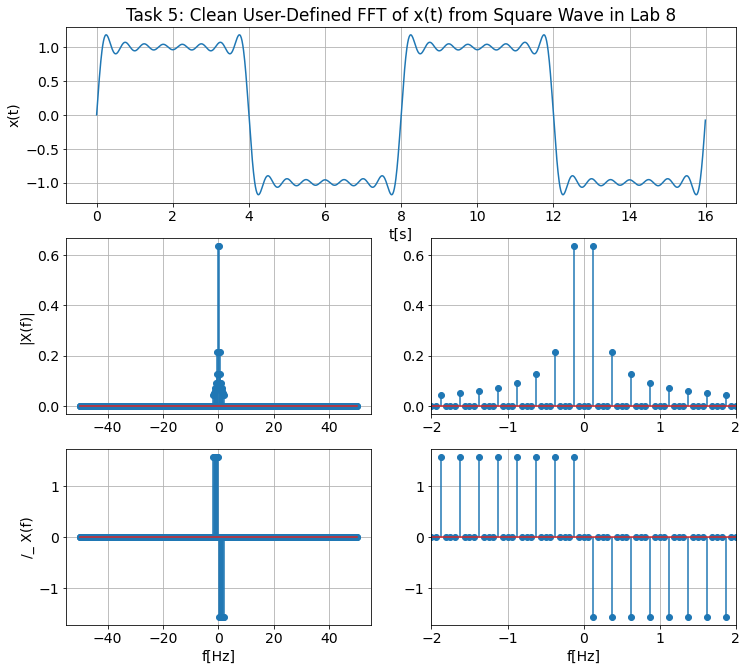
\includegraphics[scale = 0.42]{Lab 9 - Plots/Task5.png}\\[1.0 cm]
\end{center}

\section{Error Analysis}

I initially had difficulty in getting my fast Fourier transform plots to be visually distinct and readable. I first discovered that my step size was too small. I fixed this by increasing from $ 1\times 10^{-5} $ to $ 1\times 10^{-2} $. While this did make the plots more viewable, they still were not matching expectations. With the help of the TA, I discovered that the Python implementation of the fast Fourier would not work properly with my declaration of the time interval. I had to remove the addition of the step variable to the upper bound of the interval to achieve accurate results. \\  

\section{Questions}

1. If fs is lowered, the frequency domain subplots face reduced horizontal scaling. If it is higher, those subplots rather are stretched horizontally. The value of fs was held at a constant $ 100 $, as directed in the lab manual. It was replaced with $ 10 $ and $ 1000 $ to determine these behaviors. \\

2. Eliminating the small phase magnitudes removes the phases associated with points that are not contributing greatly to the frequency domain function. This results in a cleaner phase plot without greatly reducing the accuracy. \\

3. The Fourier transforms of cosine and sine are provided below alongside the transforms of Equations 1 and 2 shown also in Equations 5 and 6. 

\begin{equation*}
	\mathcal{F}\{cos(2\pi f_0t)\} = \frac{1}{2}[\delta(f - f_0) + \delta(f + f_0)]
\end{equation*}
\begin{equation*}
	\mathcal{F}\{cos(2\pi t)\} = \frac{1}{2}[\delta(f - 1) + \delta(f + 1)] 
\end{equation*}
\begin{equation*}
	\mathcal{F}\{sin(2\pi f_0t)\} = \frac{1}{j2}[\delta(f - f_0) - \delta(f + f_0)]
\end{equation*}
\begin{equation*}
	\mathcal{F}\{5sin(2\pi t)\} = \frac{5}{j2}[\delta(f - 1) - \delta(f + 1)]
\end{equation*}

The plots in Tasks 1 and 2 show Fourier transforms with magnitudes given by two delta functions, one shifted left by $ 1 $ and the other right by $ 1 $. In Task 1 the delta functions each have a magnitude of $ 0.5 $, while in Task 2 they have magnitudes of $ 2.5 $. Looking at Equation 5, the expression shows two delta functions of the same magnitude and shift as in Task 1. Similarly, Equation 6 shows two delta functions with magnitude $ 2.5 $ like in Task 2. Because the magnitude involves the absolute value function, the negative sign will not affect the result. The imaginary nature does influence the phase. Consequently, the phase subplot of Task 2 includes more points as we would expect. These close correlations between the mathematical transforms and their plots suggest that the plots found in Tasks 1 and 2 are correct. \\

4. The lab tasks, expectations, and deliverables were all presented clearly. \\

\section{Conclusion}

In this lab we learned how to implement a Fourier transform function in Python using the fast Fourier method. We practiced understanding the frequency domain magnitudes and phases of sinusoidal input functions. We gained familiarity with arranging subplots and their labels as well as limiting axes to view a section of interest. This lab also revealed how reducing minute magnitude phases increases visibility without compromising accuracy. \\

If this lab were to be repeated, I would update the lab manual to comment on how the step variable in the time interval assignment must be altered to accommodate the fast Fourier transform in Python. This is something that seems unrealistic to expect students to intuit or discover individually. Through the lab, I was able to better develop my skills in creating reusable code segments. I implemented the clean requirement as a passable argument and created a single function to plot the transforms. The ability to consolidate code will improve readability and better the quality of future assignments.

\newpage
\begin{thebibliography}{111}
	
	\bibitem{S}
	Sullivan, Dennis M. (2018) {\it  Signals and Systems for Electrical Engineers I}. Nevada: CreateSpace Independent Publishing Platform.
	
\end{thebibliography}
\end{document}

% Lab Report based on template created by Roza Aceska.